\section{Propositional logic}

I'm going to assume that you're comfortable with basic propositional logic from
other courses. If you did \texttt{COMP21111} then you're probably going to find
this easy!

Just to jog your memory, here are some PL things you should know:

\begin{itemize}
  \item A formula is \textit{satisfiable} if there exists an assignment such 
  that the formula evaluates to \texttt{T}. E.g. $p \vee q$ is \texttt{T} when $
  p = 1, q = 0$, and therefore is satisfiable. $p \wedge \neg p$ is obviously 
  not satisfiable.

  \item We can define the problem \texttt{Propositional Sat} which will 
  determine whether a given formula is satisfiable or not. Since it is possible 
  to turn any PL formula into one of the `normal forms', we need only consider 
  formula made completely from negations and disjunctions, since all other 
  formulae can be converted into something like them.

  \item Since converting a formula into normal form gives us a set of clauses, 
  we need to define the problem \texttt{SAT} which when given a set of clauses, 
  will determine whether the whole set of clauses is satisfiable (they must all 
  be satisfiable with the same truth assignment).

  \item Similarly, \texttt{k-SAT} is the problem where each clause has at most
  $k$ literals.

  \marginpar{Horn satisfiability is actually \texttt{PTime-Complete} (see 
  Section~\ref{sec:reduce-and-hard}), since we can convert any deterministic TM 
  into a set of Horn clauses.}

  \item Horn clauses are clauses where there is only 0 or one non-negative 
  literals. In other words, all but at most one literals are negative, e.g.
  $\neg x \vee \neg y \vee \neg z$ or $\neg x \vee y \vee \neg z$

  \item Krom clauses have at most two literals, e.g. $x \vee y$.
\end{itemize}

\subsection{DPLL}

The Davis-Putnam-Logemann-Loveland algorithm solves \texttt{SAT}. Here it is:

\begin{verbatim}
  begin DPLL(clauses)
    if clauses is empty then return Yes
    if clauses contains the empty clause then return No
    while clauses contains any unit clause l
      remove l from clauses
      clauses = resolve(Γ, l)
      if clauses is empty then return Yes
      if clauses contains the empty clause then return No
    let l be the first literal of the first clause of clauses
    if DPLL(clauses + l} then return Yes
    if DPLL(clauses + l} then return Yes
    return No

  begin resolve(clauses, l)
    for each x in clauses
      if x contains l, remove x from Γ
      if x contains not l, remove not l from x
\end{verbatim}

DPLL tries all the different combinations of truth assignments, and as a result,
runs in exponential time. This is close to the best way of solving \texttt{SAT}
in practice, but in practice, we don't have non-deterministic Turing machines...

\subsection{NPTime SAT}

We've shown that \texttt{SAT} is in \texttt{ExpTime} by giving an algorithm for
it, but we can also make a non-deterministic algorithm to solve it:

\begin{verbatim}
  begin NdSatTest(clauses)
    If clauses contains FALSE, then return No
    While clauses is not empty:
      Select a literal in clauses, p
      Either:
        Delete every clause containing p
        Delete not p from all the other clauses
      Or:
        Delete every clause containing not p
        Delete p from all the other clauses
      If clauses contains FALSE, then return No
    return Yes
\end{verbatim}

This is obviously in \texttt{NPTime}.

\subsection{Horn SAT}

If we have a set of Horn clauses, how does that affect \texttt{SAT}? Well, we
can in fact solve it in $O(n^2)$ time:

\begin{verbatim}
  begin Horn-DPLL(clauses)
    if clauses contains the empty clause then return No
    while clauses contains any unit clause l
      remove l from clauses
      clauses = resolve(clauses, l)
      if clauses contains the empty clause then return No
    return Yes

  begin resolve(clauses, l)
    for each x in clauses
      if x contains l, remove x from Γ
      if x contains not l, remove not l from x
\end{verbatim}

\subsection{2-SAT}

If we're given Krom clauses, we can also solve that in $O(n^2)$. To do this, you
create a graph with $2n$ nodes, one for each literal and one for its negation.
For the clauses $(x \vee y), (\neg x \vee z), (y \vee \neg z)$, we create a
graph like this:

\begin{figure}[H]
  \centering
  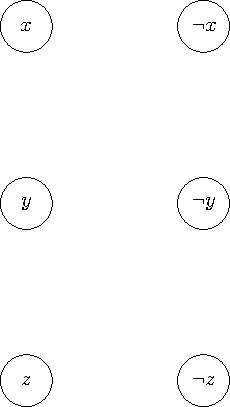
\includegraphics[width=0.2\textwidth]{diagrams/graph9}
  \caption{Initial graph for $x, \neg x, y, \neg y, z, \neg z$}
  \label{fig:graph-9}
\end{figure}

For each clause, we insert two edges. If the clause is $(a \vee b)$, we insert
$\neg a \rightarrow b$ and $\neg b \rightarrow a$:

\begin{figure}[H]
  \centering
  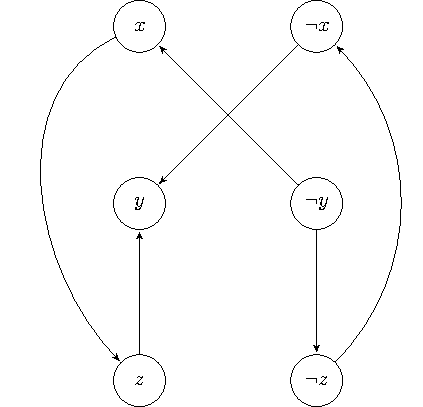
\includegraphics[width=0.35\textwidth]{diagrams/graph10}
  \caption{Graph of $x, \neg x, y, \neg y, z, \neg z$, with the appropriate
  edges.}
  \label{fig:graph-10}
\end{figure}

Then, for each node in the graph, see if there is a path to its inverse. If
there is, then the clause is \textit{unsatisfiable}. This runs in $O(n^2)$ time,
since finding a path takes $O(n)$ time, and we have to do it for each clause, so
we have to do it $n$ times.
